\overlays{5}{
\begin{slide}{Layout del sistema operativo}
A differenza di Windows, GNU/Linux non è un sistema operativo "tutto in
uno":

\begin{itemize}
	\onlySlide*{2}{\item[-]I programmi sono parte separata dal sistema}
	\onlySlide*{3}{\item[-]L'interfaccia grafica è parte separata del sistema }
	\onlySlide*{4}{\item[-]Il filesystem non è parte del sistema operativo}
\end{itemize}


\onlySlide*{5}{
\flushright{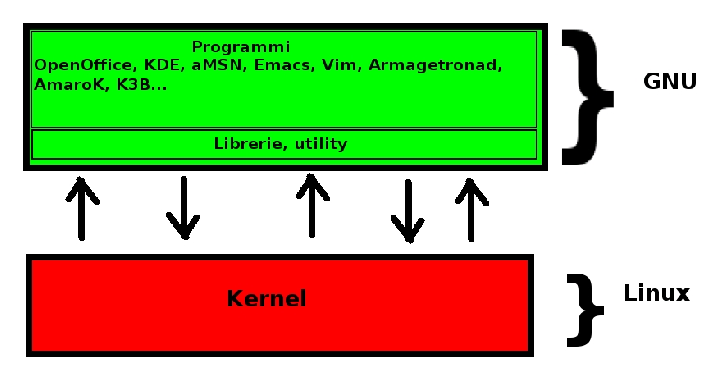
\includegraphics[width=8cm,height=6cm]{immagini/linux_layout.eps}}
}

\end{slide}
}
